\documentclass[../slides.tex]{subfiles}

\title{2018-2019 Inleiding Logica (KI1V13001) \\ Lecture 4}
 
\date{September 10, 2019\\[2ex] {\tiny \textcopyright~The non-copyrighted content of these slides is open access under \href{https://creativecommons.org/licenses/by-sa/4.0/}{CC BY-SA 4.0}}}
 
%%%%%%%%%%%%%%%

\begin{document}

\setcounter{framenumber}{97}
\begin{frame}
	\maketitle
\end{frame}

\begin{frame}[noframenumbering, plain]
\begin{center}
			\begin{tabular}{c}
			 	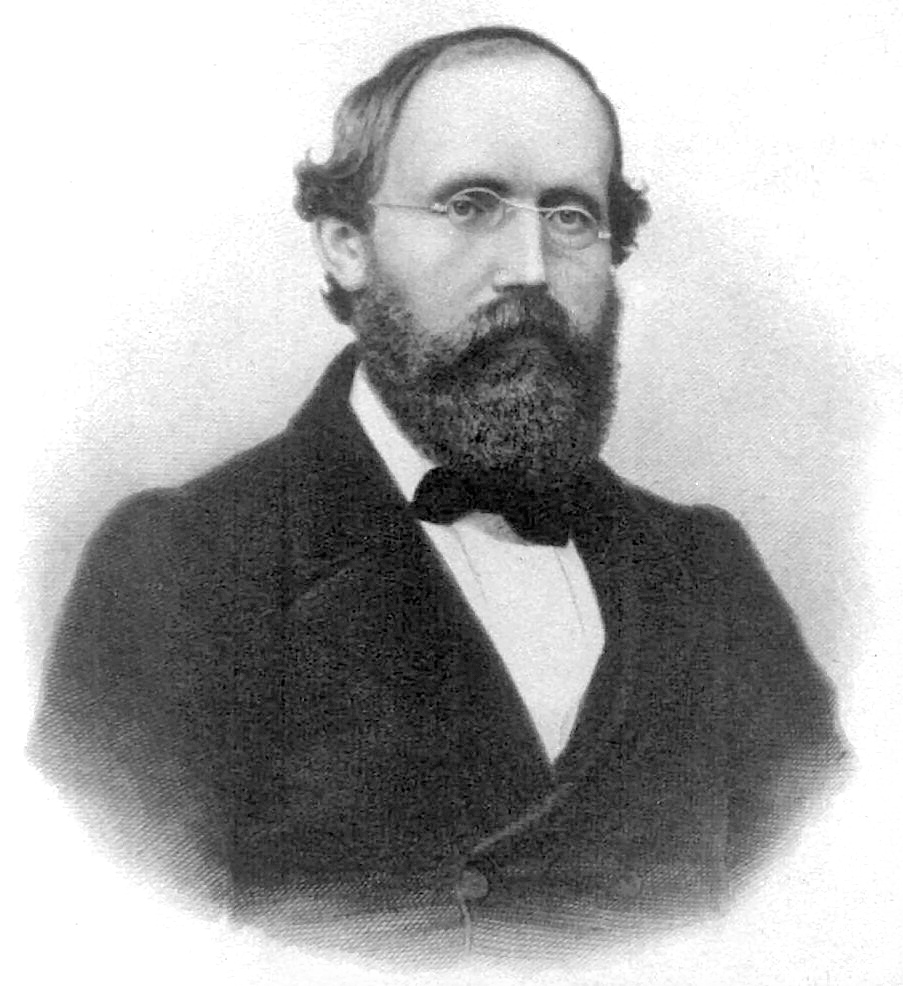
\includegraphics[height=40ex]{birthday}\\
				Georg Friedrich Bernhard Riemann\\
				Born 17 September, 1826\\
				{\tiny $\not\hspace{-1ex}\textcopyright$ work in public domain} 
			\end{tabular}
		\end{center}	

\end{frame}

\begin{frame}{Overview}
\tableofcontents
\end{frame}

\section{Rehash}
\begin{frame}{Rehash}
	
\begin{itemize}

		\item A set is a collection of objects, its elements.
		
		\item One set is a subset of another just in case all the elements of the one set are elements of the other. 
				
		\item Two sets are identical iff they have precisely the same elements. 
		
		\item The union of two sets contains any element of either set, their intersection contains only the objects that are in both sets. The difference of one set and another contains all the elements of the one but not the other.
		
		\item An ordered tuple is a a set-like collection of objects with a specific order. In tuples, order and multiplicity count.
		
		\item The Cartesian product of two sets contains all the tuples formed from those sets.
		
		\end{itemize}
		
	\end{frame}
		
\begin{frame}{Rehash (Cont'd)}
	
\begin{itemize}
			
		\item A property is a set of objects. An $n$-ary relation is a set of $n$-tuples.
		
		\item A function assigns to each input a \emph{unique} output.
		
		\item \alert{To inductively define a set, we give a set of initial elements and a set of constructions for new elements.}
		
		\item \alert{To recursively define a function, we give the value of the function for the initial elements and say how to calculate the value of a newly constructed element based on the values of the elements its constructed from.}
		
		\item \alert{To prove a claim by induction over an inductively defined set, we show that all initial element satisfy the claim and that every newly constructed element satisfies the claim whenever the elements that it's constructed from do.}
			

	\end{itemize}

\end{frame}

\section{4.0 Syntax of Propositional Logic}
\subsection{4.1 Propositional Languages}

\begin{frame}{4.1 Propositional Languages}


	\begin{itemize}
	
		\item (4.1.1) Remember that we arrive at formal languages by abstracting away from the logically irrelevant aspects of ordinary language.
		
		\item In propositional logic, what's relevant are the connectives ``not,'' ``and,'' ``or,'' ``if \dots, then \dots,'' and ``iff.''
	
		\item (4.1.2) For validity in propositional logic, concrete sentences don't matter:
	\begin{enumerate}[(1)]
		
			\item The letter is either in the left drawer or in the right drawer, and it's not in the left drawer. So, the letter is in the right drawer.
		
		\end{enumerate}
	\begin{enumerate}[(1')]
		
			\item The cat is either on the mat or the dog dances tango, and the cat isn't on the mat. So, the dog dances tango.
		
		\end{enumerate}
		
		\item So we abstract away from them.
	
	
	\end{itemize}
		
\end{frame}

\begin{frame}{Vocabulary}

	\begin{itemize}
	
		\item (4.1.4) To define a formal language, we need to define the symbols (vocabulary) and the grammar (inductive definition).
		
		\item (4.1.5) The vocabulary of a propositional language $\mathcal{L}$ contains:		
		\begin{enumerate}[(i)]
		
			\item a (non-empty) set $\mathcal{P}$ of sentence letters,
						
			\item the \emph{sentential operators} $\neg,\land,\lor,\to,$ and $\leftrightarrow$, and 
			
			\item the \emph{parentheses} $($ and $)$.
		
		\end{enumerate}

		\begin{center}
			\begin{tabular}{c | c | c}
			Symbol & Name & Reading\\ \hline
			
			$\neg$ & Negation & not\\
			$\land$ & Conjunction & and\\
			$\lor$ & Disjunction & or\\
			$\to$ & Conditional & if \dots, then \dots\\
			$\leftrightarrow$ & Biconditional & iff
			\end{tabular}
		\end{center}	
	\end{itemize}

\end{frame}

\begin{frame}{Grammar}
	
	\begin{itemize}
	
		 \item \alert{To inductively define a set, we give a set of initial elements and a set of constructions for new elements.}
		 
		 \item Initial elements=$\mathcal{P}$ and constructions=$\neg,\land,\lor,\to,\leftrightarrow$.

		\item (4.1.6) $\mathcal{L}$ is the smallest set $X$, such that:
		\begin{enumerate}[(i)]
		
			\item $\mathcal{P}\subseteq X$
			
			\item \begin{enumerate}[(a)]

					\item if $\phi\in X$, then $\neg \phi\in X$
					
					\item if $\phi,\psi\in X$, then $(\phi\land\psi), (\phi\lor\psi),(\phi\to\psi),(\phi\leftrightarrow\psi)\in X$.
		
				\end{enumerate}
					
		\end{enumerate}
				
		\item  (4.1.7) Backus-Naur-Form:
				
		\begin{center}
		$\phi::=p~|~\neg \phi~|~(\phi\land\phi)~|~(\phi\lor\phi)~|~(\phi\to\phi)~|~(\phi\leftrightarrow\phi)$
		\end{center}
		
		\item (4.1.9) \emph{Example}: 
			\begin{itemize}
				\item $q,r\in\mathcal{P}$ $\Rightarrow$ $q,r\in\mathcal{L}$ (i)
				
				\item $q,r\in\mathcal{L}$ $\Rightarrow$ $(q\lor r)\in\mathcal{L}$ (ii.b). 
				
				\item $p\in\mathcal{P}$ $\Rightarrow$ $p\in\mathcal{L}$ (i)
				
				\item $p\in\mathcal{L}$ and $(q\lor r)\in\mathcal{L}$ $\Rightarrow$ $(p\land (q\lor r))\in\mathcal{L}$ (ii.b)
		
			\end{itemize}
		
	\end{itemize}
		
\end{frame}

\begin{frame}{Exclusion}

	\begin{itemize}

		\item (4.1.9) \textbf{Proposition}. Let $\mathcal{L}$ be a propositional language. Then $(p\land \neg)\notin\mathcal{L}$.

		\item \emph{Proof} (Sketch).

		Let $X$ be a set such that $X$ satisfies conditions (i) and (ii) from the definition of $\mathcal{L}$ and $(p\land \neg)\in X$. Then also \[Y=X\setminus \{(p\land \neg), \neg\}\] satisfies the conditions but is smaller. So $X\neq \mathcal{L}$. So for proof by contradiction, suppose that $(p\land \neg)\in\mathcal{L}$. It would follow that $\mathcal{L}\neq\mathcal{L}$, which is a contradiction. Hence $(p\land \neg)\notin\mathcal{L}$. 
		
		\begin{flushright}
		$\qedsymbol$
		\end{flushright}
		

	\end{itemize}

\end{frame}

\begin{frame}{Formalization}

	\begin{itemize}
	
		\item (4.1.10) Formalization is the process of abstracting ordinary language into a formal language.
		
		\item We need a translation key which tells us what the $\mathcal{P}$'s stand for:
		
			\begin{center}
	\begin{tabular}{c c c}
	$p$ & : & the letter is in the left drawer\\
	$q$ & : & the letter is in the right drawer
	\end{tabular}
	\end{center}
	
		\item Aim: Find a formula $\phi$ that captures what the language says. 
	
	\end{itemize}

\end{frame}		

\begin{frame}{Guidelines}

\begin{tabular}{p{6cm} c c}
	The letter \alert{isn't} in the left drawer & $\leadsto$ & $\neg p$\\[1ex]
	The letter is in the left \alert{and} in the right drawer & $\leadsto$ & $(p\land q)$\\[1ex]
	The letter is not in the left drawer, \alert{but} it's also not in the right one & $\leadsto$ & $(\neg p\land \neg q)$\\[1ex]
	The letter is (\alert{either}) in the left \alert{or} in the right drawer & $\leadsto$ & $(p\lor q)$\\[1ex]
	The letter is \alert{either} (!) in the left \alert{or} in the right drawer & $\leadsto$ & $((p\lor q)\land \neg(p\land q))$\\[1ex]
	The letter is \alert{neither} in the left \alert{nor} in the right drawer  & $\leadsto$ & $(\neg p\land \neg q)$\\[1ex]
	It the letter is in the left drawer, \alert{then} it's not in the right drawer & $\leadsto$ & $(p\to \neg q)$\\[1ex]
	The letter is in the left drawer, \alert{if} it's not in the right & $\leadsto$ & $(\neg p\to q)$\\[1ex]
	The letter is \alert{only} in the left drawer, \alert{if} it's not in the right & $\leadsto$ & $(q\to \neg p)$\\
	\end{tabular}

\end{frame}
		
\subsection{4.2 Proof by Induction on Formulas}

\begin{frame}{4.2 Proof by Induction on Formulas}

	\begin{itemize}
	
		\item (4.2.1) \textbf{Theorem}. Let $\Phi$ be a condition on formulas. If we can show:
		\begin{enumerate}[(i)]
		
			\item For all $p\in\mathcal{P}$, $\Phi(p)$.
			
			\item \begin{enumerate}[(a)]
			
			\item For all $\phi\in\mathcal{L}$, if $\Phi(\phi)$, then $\Phi(\neg\phi)$.

			\item For all $\phi,\psi\in\mathcal{L}$, if $\Phi(\phi)$ and $\Phi(\psi)$, then $\Phi((\phi\circ\psi))$, for $\circ=\land,\lor,\to,\leftrightarrow$.
		
		\end{enumerate}
		\end{enumerate}
		Then we can conclude that for all $\phi\in\mathcal{L}$, $\Phi(\phi)$.
		
		\item \emph{Proof}. Let $\Phi$ be an arbitrary condition on formulas satisfying the conditions. Then also $\{x:\Phi(x)\}$ satisfies the conditions. Since $\mathcal{L}$ is the smallest set satisfying those conditions, we have that $\mathcal{L}\subseteq\{x:\Phi(x)\}$. For $\phi\in\mathcal{L}$ an arbitrary formula, it follows that $\phi\in\{x:\Phi(x)\}$. But that just means that $\Phi(\phi)$, as desired. $\qedsymbol$

	\end{itemize}


\end{frame}
		
\begin{frame}{How to Induction (4.2.2)}

	\begin{enumerate}[1.]
		
			\item State clearly that you're using induction to prove the claim.
			
			\item Prove the base case, i.e. show that all sentence letters have the property.
			
			\item State clearly that you're now considering the induction steps. In each sub-case, begin by stating your induction hypothesis and then use it to derive the claim about the constructed element, i.e.
			\begin{itemize}
			
				\item derive that $\neg\phi$ has the property from the induction hypothesis that $\phi$ has the property, and
				
				\item derive that $(\phi\circ\psi)$ has the property (for $\circ=\land,\lor,\to,\leftrightarrow$) from the induction hypotheses that $\phi$ and $\psi$ has the property.
			
			\end{itemize}
			
			\item State clearly that you're using induction to infer that the claim in question holds for all elements of the set.
		
		\end{enumerate}

\end{frame}		

\begin{frame}{Example}


	\begin{itemize}
	
		\item (4.2.4) \textbf{Proposition}. Let $\phi\in\mathcal{L}$ be a formula. Then $\phi$ contains an even number of parentheses.
		
		\item \emph{Proof}. By induction. 
				
		\begin{itemize}
	
		\item \emph{Base case}. For each $p\in\mathcal{P}$, the number of parentheses in $p$ is zero, which is an even number.
		
		\item \emph{Induction steps.}
		
		\begin{itemize}
		
			\item Suppose the induction hypothesis that $\phi\in\mathcal{L}$ contains an even number of parentheses. Consider the formula $\neg\phi$. Note the number of parentheses in $\neg\phi$ are exactly the same as in $\phi$, since no new ones have been added.
			
			\item Suppose the induction hypothesis that $\phi,\psi\in\mathcal{L}$ contain an even number of parentheses. Consider the formulas $(\phi\circ\psi)$. The number of parentheses in $(\phi\circ\psi)$ are precisely the number of parentheses in $\phi$, plus the number of parentheses in $\psi$, plus two.	 But the sum of three even numbers is even.	
		\end{itemize}
	
	\end{itemize}
		
	\item \textbf{Corollary}. Let $\phi$ be an expression. If $\phi$ contains an odd number of parentheses, then $\phi\notin\mathcal{L}$.
	
	\end{itemize}


\end{frame}

\begin{frame}

\begin{center}
		\begin{tabular}{c}
		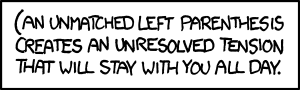
\includegraphics[width=40ex]{xkcd-(}\\[-1ex]
		{\tiny \textcopyright~\url{https://xkcd.com/859/}, CC BY-NC 2.5}
		\end{tabular}
		\end{center}

\end{frame}

\subsection{4.3 Unique Readability and Parsing Trees}

\begin{frame}{4.3 Unique Readability and Parsing Trees}

	\begin{itemize}
	
		\item (4.3.1) We want unique readability to ensure that recursion works.
		
		\item (4.3.2) We get it because of $($ and $)$:
		
	\begin{center}
		
		\begin{tabular}{c c c}
		\begin{tikzpicture}
		{\Tree [.$p\land q\lor r$ [.$p$ ] [.$q\lor r$ [.$q$ ] [.$r$ ] ] ]}
		\end{tikzpicture}

		& 
		
		\qquad \raisebox{7.5ex}{vs.} \qquad 
				\begin{tikzpicture}

		{\Tree [.$p\land q\lor r$ [.$p\land q$ [.$p$ ] [.$q$ ] ] [.$r$ ] ]}
		\end{tikzpicture}

		\end{tabular}
		\end{center}
		
		\item That's the difference between:
		\begin{itemize}
	
		\item I have a coffee and either toast or eggs.
		
		\item Either I have a coffee and toast or I have eggs.
	
	\end{itemize}
	
	\end{itemize}

\end{frame}

\begin{frame}{Trees (4.3.3)}

	\begin{center}
		\begin{tabular}{c}
		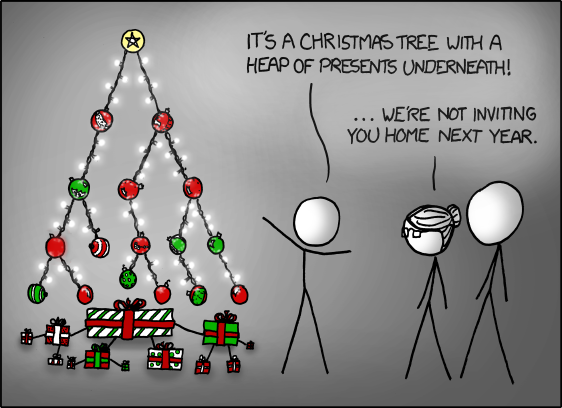
\includegraphics[width=30ex]{xkcd-tree}\\[-1ex]
		{\tiny \textcopyright~\url{https://xkcd.com/835/}, CC BY-NC 2.5}
		\end{tabular}
		\end{center}

	\begin{itemize}
		
		\item The dots (ornaments, presents) are {\it nodes}, the lines {\it edges}. 
		
		\item The upper-most node is the {\it root}, the lower-most nodes {\it leaves}. 
		
		\item If $y$ is directly above $x$, then $x$ is a {\it child} of $y$ and $y$ the \emph{parent} of $x$. 
		
		\item A {\it path} in the tree is a sequence of nodes connected by edges. 
		
		\item No loops!
		
	\end{itemize}

\end{frame}

\begin{frame}{Parsing Trees}

	\begin{itemize}
	
 		\item \alert{To recursively define a function, we give the value of the function for the initial elements and say how to calculate the value of a newly constructed element based on the values of the elements its constructed from.}
		
		\item (4.3.5) The function $T:\mathcal{L}\to Trees$ is defined by:
		
		\begin{center}
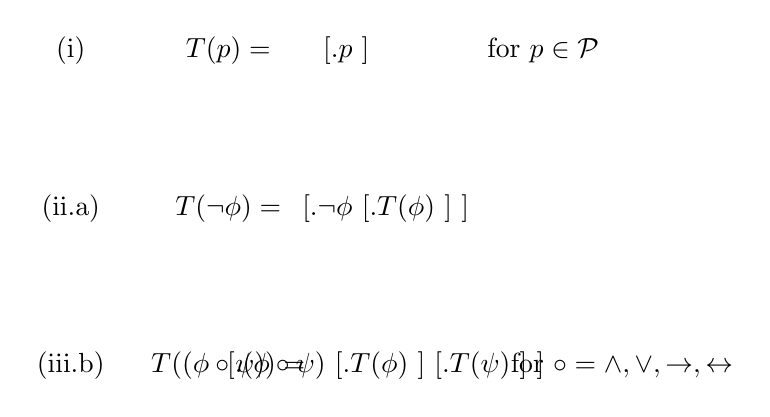
\begin{tikzpicture}
\node at (-2,1) {(i)};

\node at (0,1) {$T(p)=$};
\node at (1.5,1) {\Tree [.$p$ ]};
\node at (4,1) {for $p\in\mathcal{P}$};

\node at (-2,-1) {(ii.a)};
\node at (0,-1) {$T(\neg \phi)=$};
\node at (2,-1) {\Tree [.$\neg \phi$ [.$T(\phi)$ ] ]};

\node at (-2,-3) {(iii.b)};
\node at (0,-3) {$T((\phi\circ\psi))=$};
\node at (2,-3) {\Tree [.$(\phi\circ\psi)$ [.$T(\phi)$ ] [.$T(\psi)$ ] ]};
\node at (5,-3) {for $\circ=\land,\lor,\to,\leftrightarrow$};
\end{tikzpicture}
\end{center}

	\end{itemize}


\end{frame}

\begin{frame}{Example}

\begin{center}
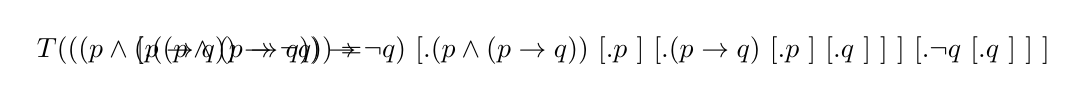
\begin{tikzpicture}
\node at (0,0) {$T(((p\land (p\to q)) \to \neg q))=$};
\node at (5,0) {\Tree [.$((p\land (p\to q))\to \neg q)$ [.$(p\land (p\to q))$ [.$p$ ] [.$(p\to q)$ [.$p$ ] [.$q$ ] ] ] [.$\neg q$ [.$q$ ] ] ]};

\end{tikzpicture}

Main operator: $\to$
\end{center}

\end{frame}

\begin{frame}{Unique Readability Theorem}

	\textbf{Theorem}. For each formula $\phi\in\mathcal{L}$ there exists a unique parsing tree, $T(\phi)$ as defined by (4.3.5).

	\begin{itemize}
	
		\item Is proven in two parts, existence and uniqueness.
		
		\item Proven in the notes (4.3.8).
		
		\item Of fundamental importance to applicability.
	
	\end{itemize}


\end{frame}

\begin{frame}{Algorithms}

\begin{center}
		\begin{tabular}{c}
		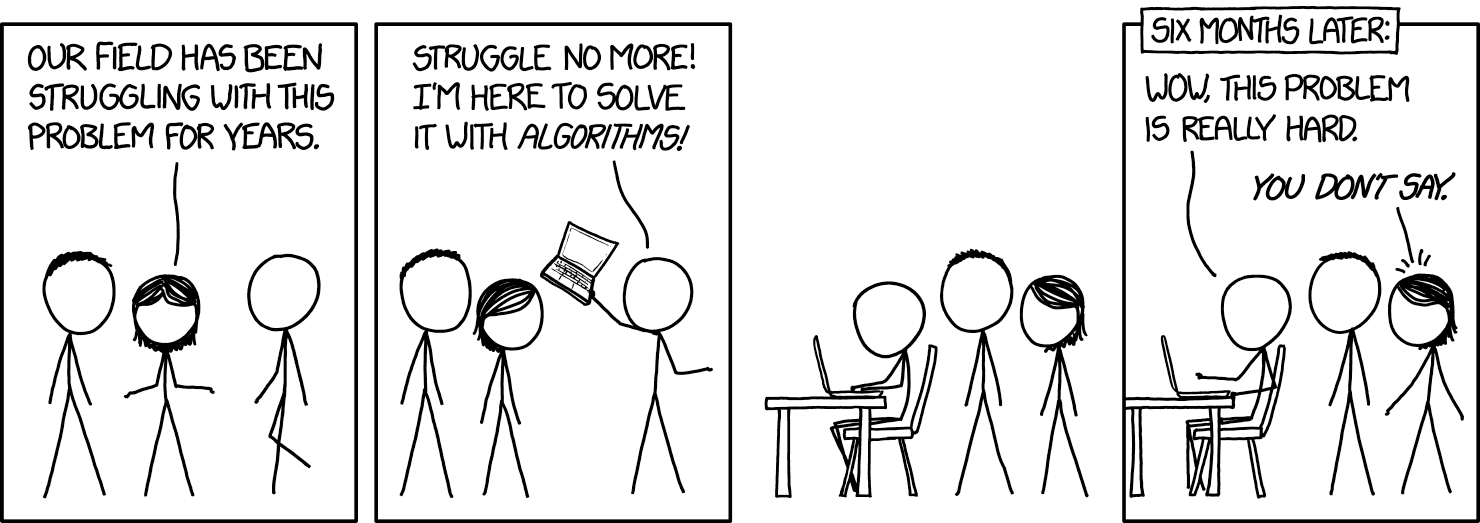
\includegraphics[width=35ex]{xkcd-algorithm}\\[-1ex]
		{\tiny \textcopyright~\url{https://xkcd.com/1831/}, CC BY-NC 2.5}
		\end{tabular}
		\end{center}

	\begin{itemize}
	
		\item (4.3.9) An algorithm is a finite set of precise instructions for a specific task. 
	
		\item We don't program, we describe algorithms abstractly.
	
	\end{itemize}

\end{frame}

\begin{frame}{The Algorithm}


\begin{enumerate}[1.]
			
				\item Write down the expression $\sigma$ and look at it. Proceed to step 2.
				
				\item Does the expression you're currently looking at contain the same number of $($'s and $)$'s?
				\begin{enumerate}[(a)]
				
					\item If not, terminate: $\sigma$ is not a formula!
					
					\item If yes, proceed to step 3.
				
				\end{enumerate}
				
				\item Is the expression you're currently looking at of the form $p$?
				
				\begin{enumerate}[(a)]
				
					\item If not, proceed to step 4.
				
					\item If yes, write a $\checkmark$ next to it and proceed to step 6.
					
				\end{enumerate}
				
				\item Is the expression you're currently looking at of the form $\neg \tau$?

				\begin{enumerate}[(a)]
				
					\item If not, proceed to step 5.

					
					\item If yes, apply the following rule:
					\begin{center}
					\Tree [.$\neg \tau\checkmark$ [.$\tau$ ] ]
					\end{center}
					Then proceed to step 6.
										
				
				\end{enumerate}
										
	
		\end{enumerate}

\end{frame}

\begin{frame}{Algorithm (Cont'd)}

	\begin{enumerate}[1.]
	\setcounter{enumi}{4}
	
	\item Is the expression you're currently looking at of the form $(\tau\circ\pi)$, $\circ=\land,\lor,\to,\leftrightarrow$, \emph{and} there is no other connective $\square=\land,\lor,\to,\leftrightarrow$ such that the expression is of the form $(\tau'\square\pi')$?				
	
			\begin{enumerate}[(a)]
		
				\item If not, terminate: $\sigma$ is not a formula!
				
				\item If yes, apply the following rule:
			
				\begin{center}
				\Tree [.$(\tau\circ\pi)\checkmark$ [.$\tau$ ] [.$\pi$ ] ]
				\end{center}
			
				Then proceed to step 6.	
			
			\end{enumerate}
		
			\item In the tree you've constructed so far, is there an expression at a leaf without a $\checkmark$ next to it?
		
			\begin{enumerate}[(a)]
			
				\item If no, terminate: $\sigma$ is a formula \smiley		
				
				\item If yes, then pick one and look at it. Go back to step 2.
			
		
			\end{enumerate}
			
		\end{enumerate}

\end{frame}

\begin{frame}{Example \smiley}

	\begin{center}
	\Tree[.$(p\lor (q\lor (r\leftrightarrow (\neg s\land t))))\checkmark^{5.b}$ [.{$p\checkmark^{3.b}$} ] [.{$(q\lor (r\leftrightarrow (\neg s\land t)))\checkmark^{5.b}$} [.{$q\checkmark^{3.b}$} ] [.{$(r\leftrightarrow (\neg s\land t))\checkmark^{5.b}$} [.$r\checkmark^{3.b}$ ] [.$(\neg s\land t)\checkmark^{5.b}$ [.$\neg s\checkmark^{4.b}$ [.$s\checkmark^{3.b}$ ] ] [.$t\checkmark^{3.b}$ ] ] ] ] ]
	\end{center}
	
\end{frame}

\begin{frame}{Examples \frownie}

\begin{center}		
\begin{tabular}{c c c}
				\Tree [.$((p\land q)\to \neg(r))\checkmark^{5.b}$ [.$(p\land q)\checkmark^{5.b}$ [.$p\checkmark^{3.b}$ ] [.$q\checkmark^{3.b}$ ] ] [.$\neg(r)\checkmark^{4.b}$ [.$(r)\frownie^{5.a}$ ] ] ] 
			
			& \qquad &
			
				\Tree [.${\neg\neg(p(\leftrightarrow) q)}\checkmark^{4.b}$ [.${\neg(p(\leftrightarrow) q)}\checkmark^{4.b}$ [.${(p(\leftrightarrow) q)}\checkmark^{5.b}$ [.$(p(\frownie^{2.a}$ ] [.$)q)\frownie^{2.a}$ ] ] ] ]
				\end{tabular}
				\end{center}

\end{frame}

\subsection{4.4 Function Recursion on Propositional Languages}

\begin{frame}{4.4 Function Recursion on Propositional Languages}


	\begin{itemize}
	
 		\item \alert{To recursively define a function, we give the value of the function for the initial elements and say how to calculate the value of a newly constructed element based on the values of the elements its constructed from.}
		
		\item (4.4.2) The set of sub-formulas of $\phi$ is denoted $sub(\phi)$:
		\begin{enumerate}[(i)]
		
			\item $sub(p)=\{p\}$ for $p\in\mathcal{P}$
			
			\item \begin{enumerate}[(a)]
			
				\item $sub(\neg\phi)= sub(\phi)\cup\{\neg \phi\}$
				
				\item $sub((\phi\circ\psi))= sub(\phi)\cup sub(\psi)\cup\{(\phi\circ\psi)\}$
			
			\end{enumerate}
			\end{enumerate}
			
		\item \emph{Examples}.
		
		\begin{itemize}
		
			\item $sub(\neg \neg p)=\{p,\neg p, \neg\neg p\}$
			
			\item $sub(((p\land q)\lor r))=\{p,q,r,(p\land q), ((p\land q)\lor r)\}$
		
		\end{itemize}
		
		\item (4.4.3) \textbf{Proposition}. Let $\phi\in\mathcal{L}$ be a formula. The elements of $sub(\phi)$ are precisely the formulas that occur in $T(\phi)$.
		
		\item Proved in the notes (using \dots?) 
	\end{itemize}

\end{frame}

\begin{frame}{Complexity}

		\begin{itemize}
	
 		\item \alert{To recursively define a function, we give the value of the function for the initial elements and say how to calculate the value of a newly constructed element based on the values of the elements its constructed from.}
		
		\item The \emph{complexity} of $\phi$ is denoted $c(\phi)$:
		 \begin{enumerate}[(i)]
	
		\item $c(p)=0$ for $p\in\mathcal{P}$
		
		\item \begin{enumerate}[(a)]
		
			\item $c(\neg\phi)=c(\phi)+1$
			
			\item $c((\phi\circ\psi))=max(c(\phi), c(\psi))+1$, for $\circ=\land,\lor,\to,\leftrightarrow$.
		
		\end{enumerate}
		\end{enumerate}
		
		
		\item \emph{Examples}.
		
		 \begin{itemize}
	
		\item $c(\neg p)=1$, $c((p\land q))=1, c((p\lor q)=1, \mathellipsis$
		
		\item $c(\neg\neg p)=2$, $c(\neg (p\land q))=2$, $c((\neg p\land \neg q))=2, \mathellipsis$
	
	\end{itemize}
		
		
		\end{itemize}

\end{frame}

\begin{frame}{Theorem 4.4.5}

	\begin{itemize}
	
		\item \textbf{Proposition}. Let $\phi\in\mathcal{L}$ be a formula. Then $c(\phi)$ is the length of the longest path in $T(\phi)$ which starts from the root (counted in number of edges travelled).
		
		\item \emph{Proof}. By \dots ?
		
		\begin{enumerate}[(i)]
		
			\item \emph{Base case}. For $p\in\mathcal{P}$, $T(p)=p$, which only has the trivial path. Since $c(p)=0$, we're good.
			
			\item \emph{Induction steps}. 
				\begin{enumerate}[(a)]

					\item Assume the induction hypothesis that $c(\phi)$ is the length of the longest path from the root in $T(\phi)$. By the (ii.a) definition of parsing trees, we know that:
					\begin{center}
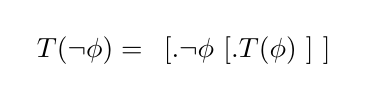
\begin{tikzpicture}
\node at (0,0) {$T(\neg \phi)=$};
\node at (2,0) {\Tree [.$\neg \phi$ [.$T(\phi)$ ] ]};
\end{tikzpicture}
\end{center}
The longest path in $T(\neg\phi)$ is the longest path in $T(\phi)$ plus one edge to $\neg\phi$. Since $c(\neg\phi)=c(\phi)+1$, we're golden.
		
		\end{enumerate}
		
		\end{enumerate}
	
	\end{itemize}

\end{frame}
\begin{frame}{Proof (Cont'd)}

\begin{enumerate}[(i)]
		
			\item \emph{Base case}. \checkmark
			
			\item \emph{Induction steps}. 
				\begin{enumerate}[(a)]

					\item \checkmark
					
					\item Assume the induction hypotheses that $c(\phi)$ is the length of the longest path from the root in $T(\phi)$ and $c(\psi)$ is the length of the longest path from the root in $T(\psi)$. By (ii.a):
					\begin{center}
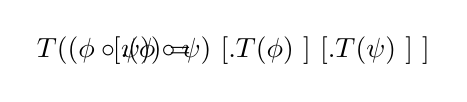
\begin{tikzpicture}
\node at (0,0) {$T((\phi\circ\psi))=$};
\node at (2,0) {\Tree [.$(\phi\circ\psi)$ [.$T(\phi)$ ] [.$T(\psi)$ ] ]};
\end{tikzpicture}
\end{center}
The longest path in $T((\phi\circ\psi))$ is the longest path you can find in either $T(\phi)$ or $T(\psi)$ plus the one new edge connecting $T(\phi)$ to the new root $(\phi\circ\psi)$. Since $c((\phi\circ\psi))=max(c(\phi),c(\psi))+1$, we're done. 

		
		\end{enumerate}
		
		\item[] $\qedsymbol$
		
		\end{enumerate}
	
\end{frame}

\section{4.5 Some Useful Notational Conventions}

\begin{frame}{4.5 Some Useful Notational Conventions}

\emph{Outside the context of syntax theory}:

	\begin{itemize}
	
		\item (4.5.3) Outermost parentheses may be omitted: \[(p\to q)\leadsto p\to q\]
		
		\item (4.5.4) In series of $\lor$'s or $\land$'s, parentheses may be omitted:\[((p\land (q\land (r\land (s\land t)))))\leadsto p\land q\land r\land s\land t\]
	
		\item (4.5.6) We read according to binding strength: \[{\neg} <{\land}={\lor}<{\to}<{\leftrightarrow}.\]
		
			\begin{center}
		
		\begin{tabular}{c c c}
		\begin{tikzpicture}
		{\Tree [.$p\land q\to r$ [.$p$ ] [.$q\to r$ [.$q$ ] [.$r$ ] ] ]}
		\end{tikzpicture}

		& 
		
		\qquad \raisebox{7.5ex}{vs.} \qquad 
				\begin{tikzpicture}

		{\Tree [.$p\land q\to r$ [.$p\land q$ [.$p$ ] [.$q$ ] ] [.$r$ ] ]}
		\end{tikzpicture}

		\end{tabular}
		\end{center}
	
	\end{itemize}


\end{frame}

\begin{frame}{Core Ideas (Lecture Version)}
 
 
 \begin{itemize}

	\item A formal language is defined by a vocabulary (symbols) and a grammar (rules).
	
	\item The vocabulary of a propositional language consists of $\mathcal{P}$ and $\neg,\land,\lor,\to,\leftrightarrow$.
	
	\item The set $\mathcal{L}$ of formulas is the smallest set containing the sentence letters and is closed under the connectives. 
	
	\item Formalization is the process of abstracting ordinary language expressions into a propositional language.
	
	\item For syntactic recursion you specify the values the $\mathcal{P}$'s and how $\neg,\land,\lor,\to,\leftrightarrow$ affect the value.
	
	\item The parsing tree shows how a formula was constructed.
	
	\item The unique readability theorem states that every formula has a unique parsing tree.
	
	\item There is a useful algorithm for syntax checking.
	
	\item \emph{Outside of syntax}, the notational conventions are useful.

\end{itemize}


\end{frame}


\begin{frame}

	\begin{center}
	{\huge\bf Thanks!}
	\end{center}

\end{frame}

\end{document}
